\documentclass[11pt]{article}
\usepackage[hmargin=1in,vmargin=1in]{geometry}
\usepackage{xcolor}
\usepackage{amsmath,amssymb,amsfonts,url,sectsty,framed,tcolorbox,framed,graphicx,mathdesign}
\newcommand{\pf}{{\bf Proof: }}
\newtheorem{theorem}{Theorem}
\newtheorem{lemma}{Lemma}
\newtheorem{proposition}{Proposition}
\newtheorem{definition}{Definition}
\newtheorem{remark}{Remark}
\newcommand{\qed}{\hfill \rule{2mm}{2mm}}

\begin{document}
\noindent
\rule{\textwidth}{1pt}
\begin{center}
{\bf [CS304] Introduction to Cryptography and Network Security}
\end{center}
Course Instructor: Dr. Dibyendu Roy \hfill Winter 2022-2023 \\
Scribed by: Srushti Rathva (202051183) \hfill Lecture (Week 6) \\
\rule{\textwidth}{1pt}

\section*{Advanced Encryption Standard (AES)}
Winner of competition was Rijndael and winning implementation was named AES. \\
It is iterated block cipher and It is based on Substitution Permutation Network (SPN). \\

\subsection*{AES - 128}
1. Block Size = 128 bits \\
2. No. of Rounds = 10 \\
3. Secret key Size = 128 bits

\subsection*{AES - 192}
1. Block Size = 128 bits \\
2. No. of Rounds = 12 \\
3. Secret key Size = 192 bits

\subsection*{AES - 256}
1. Block Size = 128 bits \\
2. No. of Rounds = 14 \\
3. Secret key Size = 256 bits \\
\\
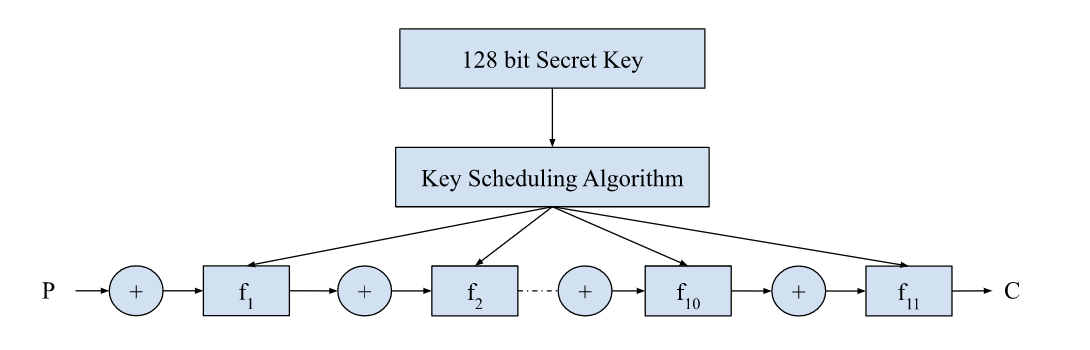
\includegraphics[width=500pt]{p1.png}
\\ \\
Mainly two things are important while implementing AES : \\
1. Round Functions \\
2. Key Scheduling Algorithm

\subsection*{Round Functions}
In \textbf{AES-128} there are \textbf{10 rounds} of encryption and corresponding to every round there is a \textbf{round function}. \\ 
$f_{1},f_{2},f_{3}$ ... $f_{10}$ \\ 
\\
\textbf{First 9 Round Functions} \\
First 9 functions are exactly same. \\
i.e $f_{1} = f_{2} = f_{3}$ ... $ = f_{9}$ \\ 
$f_{i}$ : $\{0,1\}^{128} \rightarrow \{0,1\}^{128}$ \\
\\
These 9 functions are based on following functions : \\
1. Subbytes \\
2. Shiftrows \\
3. Mix column \\
\\
$f_{i}(X)$ = $Mixcolumn(Shiftrows(Subbytes(X)))$ \\
$f_{i}^{-1}(X)$ = $Subbytes^{-1}(Shiftrows^{-1}(Mixcolum^{-1}(X)))$\\
\\
\textbf{Last Round Function} \\
Last round function $f_{10}$ is different from $f_{i}$ \\
$f_{10}$ : $\{0,1\}^{128} \rightarrow \{0,1\}^{128}$ \\
\\
The last function is based on following functions : \\
1. Subbytes \\
2. Shiftrows \\
\\
$f_{10}(X)$ = $Shiftrows(Subbytes(X))$ \\
$f_{10}^{-1}(X)$ = $Subbytes^{-1}(Shiftrows^{-1}(X))$\\

\subsection*{Subbytes}
Subbytes : $\{0,1\}^{128} \rightarrow \{0,1\}^{128}$ \\
Let $\mathcal{S} \rightarrow$ Input \\ \\
$\mathcal{S}$ = 
$
\begin{bmatrix}
\mathcal{S}_{00} & \mathcal{S}_{01} & \mathcal{S}_{02} & \mathcal{S}_{03} \\
\mathcal{S}_{10} & \mathcal{S}_{11} & \mathcal{S}_{12} & \mathcal{S}_{13} \\
\mathcal{S}_{20} & \mathcal{S}_{21} & \mathcal{S}_{22} & \mathcal{S}_{23} \\
\mathcal{S}_{30} & \mathcal{S}_{31} & \mathcal{S}_{32} & \mathcal{S}_{33} \\
\end{bmatrix}
_{4\times4}
$ \\
Here, $\mathcal{S}_{ij} \rightarrow$ 8 bits \\
\\
Let P $\rightarrow$ Plaintext \\
P = $P_{0}P_{1}...P_{15}$ \\
P $\rightarrow$ 128 bits \\
\\
Let $K_{i} \rightarrow $ Round Key \\
$K_{i}$ = $K_{0}K_{1}...K_{15}$ \\
$K_{i}$ $\rightarrow$ 128 bits \\
\\
P $\oplus$ $K_{i}$ = $\mathcal{S}$ \\
\\
$
\begin{bmatrix}
P_{0} & P_{4} & P_{8} & P_{12} \\
P_{1} & P_{5} & P_{9} & P_{13} \\
P_{2} & P_{6} & P_{10} & P_{14} \\
P_{3} & P_{7} & P_{11} & P_{15} \\
\end{bmatrix}
\bigoplus 
\begin{bmatrix}
K_{0} & K_{4} & K_{8} & K_{12} \\
K_{1} & K_{5} & K_{9} & K_{13} \\
K_{2} & K_{6} & K_{10} & K_{14} \\
K_{3} & K_{7} & K_{11} & K_{15} \\
\end{bmatrix}
=
\begin{bmatrix}
\mathcal{S}_{00} & \mathcal{S}_{01} & \mathcal{S}_{02} & \mathcal{S}_{03} \\
\mathcal{S}_{10} & \mathcal{S}_{11} & \mathcal{S}_{12} & \mathcal{S}_{13} \\
\mathcal{S}_{20} & \mathcal{S}_{21} & \mathcal{S}_{22} & \mathcal{S}_{23} \\
\mathcal{S}_{30} & \mathcal{S}_{31} & \mathcal{S}_{32} & \mathcal{S}_{33} \\
\end{bmatrix}
$ \\
\\ \\
$\mathcal{S}$ = $(\mathcal{S}_{ij})_{4\times4}$ \\
S : $\{0,1\}^{8} \rightarrow \{0,1\}^{8}$ \\
S(0) = 1 \\
\\
Given following : \\
\textbf{Special constant byte} \\
$
\begin{pmatrix}
c_{7} & c_{6} & c_{5} & c_{4} & c_{3} & c_{2} & c_{1} & c_{0}
\end{pmatrix}
=
\begin{pmatrix}
0 & 1 & 1 & 0 & 0 & 0 & 1 & 1
\end{pmatrix}_{2}
= 
\begin{pmatrix}
63
\end{pmatrix}_{16}
$ \\
\textbf{Matrix $\mathcal{S}$} \\
$\mathcal{S}_{ij}
=
\begin{pmatrix}
a_{7} & a_{6} & a_{5} & a_{4} & a_{3} & a_{2} & a_{1} & a_{0}
\end{pmatrix}
$ \\
\\
Subbytes : S(X) is defined as \\
$
b_{i} = 
(a_{i} + a_{(i+4)\%8} + a_{(i+5)\%8} + a_{(i+6)\%8} + a_{(i+7)\%8} + c_{i} )mod2 
$ \\
$S_{ij} = 
\begin{pmatrix}
b_{7} & b_{6} & b_{5} & b_{4} & b_{3} & b_{2} & b_{1} & b_{0}
\end{pmatrix}
$ \\
\\
Similarly, we'll calculate whole matrix \\
\\
$
\begin{bmatrix}
\mathcal{S}_{00} & \mathcal{S}_{01} & \mathcal{S}_{02} & \mathcal{S}_{03} \\
\mathcal{S}_{10} & \mathcal{S}_{11} & \mathcal{S}_{12} & \mathcal{S}_{13} \\
\mathcal{S}_{20} & \mathcal{S}_{21} & \mathcal{S}_{22} & \mathcal{S}_{23} \\
\mathcal{S}_{30} & \mathcal{S}_{31} & \mathcal{S}_{32} & \mathcal{S}_{33} \\
\end{bmatrix}
\rightarrow
\begin{bmatrix}
S_{00} & S_{01} & S_{02} & S_{03} \\
S_{10} & S_{11} & S_{12} & S_{13} \\
S_{20} & S_{21} & S_{22} & S_{23} \\
S_{30} & S_{31} & S_{32} & S_{33} \\
\end{bmatrix}
$ \\
\\\\
S : $\{0,1\}^{8} \rightarrow \{0,1\}^{8}$ \\
S(0) = 1 \\
$x \neq 0 \in \{0,1\}^{8} \\
S(x) = y \in \{0,1\}^{8} \\
x =
\begin{pmatrix}
a_{7} & a_{6} & a_{5} & a_{4} & a_{3} & a_{2} & a_{1} & a_{0}
\end{pmatrix} \\
a_{i} \in {0,1} \\
$ \\
Consider, \\
$
p(x) = a_{0} + a_{1}x + a_{2}x^{2} + a_{3}x^{3} + a_{4}x^{4} + a_{5}x^{5} + a_{6}x^{6} + a_{7}x^{7} \\
deg(p(x)) \leq 7 \\
p(x) \in \mathbb{F}_{2}[x] \\
p(x) \rightarrow
$ polynomial ring \\ 
\\
$
g(x) = x^{8} + x^{4} + x^{3} + x + 1 \\
g(x) \rightarrow
$ primitive polynomial \\
\\
$
\mathbb(F)_{2}[x]/<g(x)>,+,*) \rightarrow
$ Field \\
\\
Goal : Find multiplicative inverse of $p(x)$ under modulo $g(x)$ \\
$p(x)q(x) \equiv$ 1 mod$(g(x))$ \\
$p(x)q(x) - 1 = h(x)g(x)$ \\
$p(x)q(x) + h(x)g(x) = 1 $ \\
$gcd(p(x),q(x)) = 1$ \\ 
\\
We know that, $gcd(a,b) = as + bt $ \\
We'll find $q(x)$ using \textbf{extended euclidean algorithm}. \\
\\
$
p(x) = x^{6} + x^{4} + x + 1  \\
g(x) = x^{8} + x^{4} + x^{3} + x + 1 \\
$
\\
$
x^{6} + x^{4} + x + 1 \overline{)x^{8} + x^{4} + x^{3} + x + 1(} x^{2} + 1 \\
\hspace*{2.75cm} x^{8} + x^{6} + x^{3} + x^{2} \\
\hspace*{3.6cm} \overline{x^{6} + x^{4} + x^{2} + x + 1} \\
\hspace*{3.6cm} x^{6} + x^{4} + x + 1 \\
\hspace*{3.6cm} \overline{\hspace{1.65cm}x^2} \overline{) x^{6} + x^{4} + x + 1(} x^{4} + x^{2} \\
\hspace*{5.75cm} x^{6} \\
\hspace*{5.75cm} \overline{\hspace{0.75cm}x^4} \\
\hspace*{6.5cm} x^4 \\
\hspace*{6.5cm} \overline{x + 1 )x^2\hspace{0.65cm}(} x \\
\hspace*{7.5cm} x^2 + 1 \\
\hspace*{7.5cm} \overline{\hspace{0.85cm}1} \\
$ 
\\
$
1 = q(x)p(x) + h(x)g(x) \\
1 = x^{2} + (x+1)(x+1) \\
1 = x^{2} + (x+1)((x^{6}+x^{4}+x+1) + x^{2}(x^{4}+x^{2})) \\
1 = (x+1)(x^{6}+x^{4}+x+1) + [1 + (x+1)(x^{4}+x^{2})]x^{2} \\
1 = (x+1)(x^{6}+x^{4}+x+1) + (1+x^{5}+x^{4}+x^{3}+x^{2})x^{2} \\
1 = (x+1)(x^{6}+x^{4}+x+1) + (1+x^{5}+x^{4}+x^{3}+x^{2})[(x^{8}+x^{4}+x^{3}+x+1) + (x^{2}+1)(x^{6} + x^{4} + x + 1)] \\
1 = (1+x^{5}+x^{4}+x^{3}+x^{2})(x^{8}+x^{4}+x^{3}+x+1) + [(x+1) + (x^{5}+x^{4}+x^{3}+x^{2}+1)(x^{2}+1)](x^{6}+x^{4}+x+1) \\
$
\\
Coefficient  
$
= x+1+x^{2}+x^{7}+x^{4}+x^{5}+x^{4}+1+x^{5}+x^{6}+x^{3}+x^{2} \\
\hspace*{1.75cm} = x^{7}+x^{6}+x^{3}+x \\
\hspace*{1.75cm} = 
\begin{pmatrix}
1 & 1 & 0 & 0 & 1 & 0 & 1 & 0
\end{pmatrix}_{2} \\
$
\\
We'll calculate, Subbyte using below formula : \\
$
b_{i} = 
(a_{i} + a_{(i+4)\%8} + a_{(i+5)\%8} + a_{(i+6)\%8} + a_{(i+7)\%8} + c_{i} )mod2 \\
\\
\mathcal{S}(01010011) = (11001010) = 
\begin{pmatrix}
a_{7} & a_{6} & a_{5} & a_{4} & a_{3} & a_{2} & a_{1} & a_{0}
\end{pmatrix} \\
b_{0} = (0+0+0+1+1+1)\%2 = 1 \\
b_{1} = (1+0+1+1+0+1)\%2 = 0 \\
$ \\
Similarly, we'll calculate rest. \\ 
S
$(11001010) = (11101101) =
\begin{pmatrix}
b_{7} & b_{6} & b_{5} & b_{4} & b_{3} & b_{2} & b_{1} & b_{0}
\end{pmatrix}
$ 
\end{document}
